\subsection{Parte 1: circuito RLC in corrente impulsata}

Obiettivo dell'esperienza è la misura delle costanti caratteristiche del circuito RLC attraverso la rilevazione della forma d'onda del segnale di tensione, in funzione del tempo, nei tre regimi di smorzamento.

La dinamica di carica e scarica del circuito, è realizzata impostando un segnale di onda quadra con una frequenza sufficientemente bassa, in funzione dei tempi caratteristici di carica e scarica del circuito.

La rilevazione del segnale avviene con un oscilloscopio le cui sonde sono posizionate ai capi della resistenza.

La dinamica del sistema è matematicamente identica a quella di un oscillatore armonico smorzato con forzante costante, e può perciò essere convenientemente espressa anche in termini dei parametri meccanici $w_0^2$, la forza di richiamo per unità di massa e spostamento e $\gamma$, il coefficiente di smorzamento.

\begin{align*}
V_0    = & L\dot{I} + RI + Q/C   \\
0      = & \ddot{Q} + 2\gamma \dot{Q} + \omega_0^2(Q-Q_0) \\
\end{align*}

La parametrizzazione meccanicistica è stata utilizzata in fase di stima dei modelli parametrici nei tre regimi di smorzamento. 

Le stime e gli errori sui parametri elettrici sono stati ricavati successivamente usando le relazioni inverse che li legano a quelli meccanici.





%%%%%%%%%%%%%%%%%%%%%%%%%%%%%%%%%%%%%%%%%%%%%%%%%%
%%%%%%%%%%%%%%%%%%%%%%%%%%%%%%%%%%%%%%%%%%%%%%%%%%
%%%%%%%%%%% SOTTO



\subsubsection{Regime sottosmorzato}

Indicando con 
$\omega = \sqrt{\omega_0^2 - \gamma^2}$, $\gamma < \omega_0$,

\begin{align*}
V(t) / V_{0} =&  A \; e^{-\gamma t} \; [ \gamma \cos\omega t + \omega \sin\omega t ] \\
A =& RC
\end{align*}

Inteso come modello parametrico in funzione dei tre parametri incogniti $w$, $\gamma$ e $A$. $V_0$ è misurabile direttamente dal primo canale dell'oscilloscopio. L'adattamento è stato eseguito con fit non lineare sui dati

\begin{table}[H]
\begin{center}
\begin{tabular}{|c|c|c|c|}
\hline
Tempo & Ddp & Tempo & Ddp \\ \hline
$\mu s$ & $mV$ & $\mu s$ & $mV$ \\ \hline
$\pm 8$ & $\pm 16$ & $\pm 8$ & $\pm 16$ \\ \hline
0 & 0 & 412 & 352 \\ \hline
40 & 480 & 444 & 416 \\ \hline
84 & 728 & 476 & 352 \\ \hline
120 & 600 & 504 & 200 \\ \hline
160 & 224 & 532 & 0 \\ \hline
180 & 0 & 620 & -320 \\ \hline
200 & -200 & 716 & 0 \\ \hline
220 & -400 & 796 & 240 \\ \hline
264 & -560 & 972 & -184 \\ \hline
300 & -432 & 1150 & 144 \\ \hline
340 & -144 & 1330 & -104 \\ \hline
356 & 0 & 1500 & 88 \\ \hline
380 & 176 &  &  \\ \hline
\end{tabular}
\end{center}
\caption{ Sottosmorzato.
Resistenza 100 (+50+50)  [$\Omega$].
Capacità  46    [$nF$].
Induttore 0.065 [$H$].
}
\label{tab:C4_P1_sotto}
\end{table}

\begin{figure}[H]
\centering
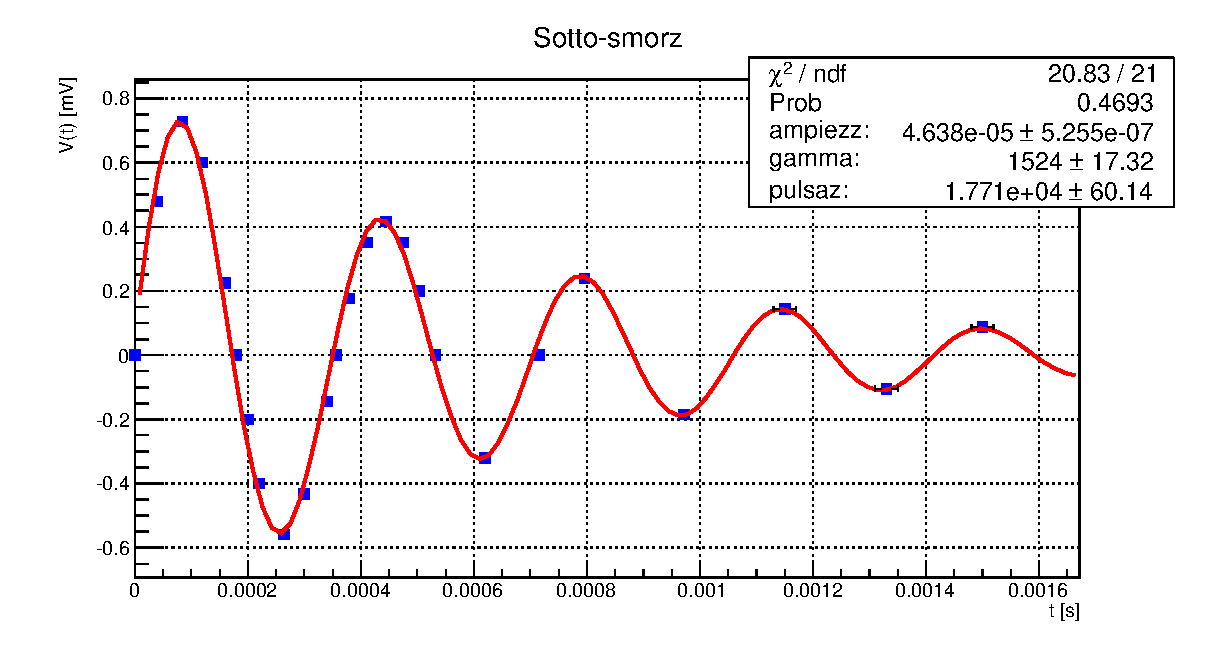
\includegraphics[scale=0.75]{Grafici/C4_P1_Sotto-smorz.eps}
\caption{
Circuito RLC serie. Regime sottosmorzato.
}
\label{fig:C4_P1_sotto}
\end{figure}

Nel regime sottosmorzato non è possibile ottenere una stima puntuale dei parametri $R$, $C$ e $L$ perchè lo jacobiano di trasformazione tra parametri elettrici e meccanici ha determinante nullo.

\begin{align*}
    A / V_0 = & RC   \\
    2\gamma    = & R/L   \\
    w_0^{-2} = (w^2+\gamma^2)^{-1}    = & RL
\end{align*}

Le alternative sono: (a) ottenere una misura diretta di $R_{tot}$ misurando la resistenza delle singole componenti con multimetro palmare. Oppure (b) combinare queste misure con altre ottenute negli altri regimi.

Qui di seguito i risultati ottenuti seguendo il metodo (a):

\begin{table}[H]
\begin{center}
\begin{tabular}{|c|c|c|c|}
\hline

Parametro & Misura & Unità & stima \\ \hline

$R_{tot}$ & diretta & $\Omega$ & $200\pm1\%$ \\ 

$C$ & indiretta & $nF$ & $46.4\pm3\%$ \\ 

$L$ & indiretta & $H$ & $0.066\pm2\%$ \\ 

\hline
\end{tabular}
\end{center}
\caption{
Misure indirette dei parametri C e L.
Regime sottosmorzato.
}
\label{C4_P1_sotto_fit}
\end{table}




%%%%%%%%%%%%%%%%%%%%%%%%%%%%%%%%%%%%%%%%%%%%%%%%%%
%%%%%%%%%%%%%%%%%%%%%%%%%%%%%%%%%%%%%%%%%%%%%%%%%%
%%%%%%%%%%% CRITICO



\subsubsection{Regime di smorzamento critico}

Alla condizione che $\omega_0 = \gamma$, il modello teorico per la ddp è

\begin{align*}
V(t)/ V_{0} =& A \gamma^{2} t e^{-\gamma t}    \\
A = & RC
\end{align*}

Inteso come modello parametrico in funzione dei due parametri incogniti $\gamma$ e $A$. $V_0$ è misurabile direttamente dal primo canale dell'oscilloscopio. L'adattamento è stato eseguito con fit non lineare sui dati


\begin{table}[H]
\begin{center}
\begin{tabular}{|c|c|c|c|}
\hline
Tempo & Ddp & Tempo & Ddp \\ \hline
$\mu s$ & $mV$ & $\mu s$ & $mV$ \\ \hline
$\pm 4$ & $\pm 80$ & $\pm 4$ & $\pm 80$ \\ \hline
0 & 0 & 74 & 6920 \\ \hline
4 & 1320 & 84 & 6520 \\ \hline
8 & 2480 & 100 & 5880 \\ \hline
12 & 3400 & 124 & 4760 \\ \hline
18 & 4560 & 150 & 3640 \\ \hline
24 & 5480 & 185 & 2400 \\ \hline
34 & 6520 & 210 & 1720 \\ \hline
44 & 7040 & 234 & 1240 \\ \hline
51 & 7200 & 310 & 440 \\ \hline
54 & 7280 & 402 & 120 \\ \hline
64 & 7160 & \multicolumn{1}{l|}{} & \multicolumn{1}{l|}{} \\ \hline
\end{tabular}
\end{center}
\caption{Smorzamento critico.
Resistenza 2390 (+50+50)   [$\Omega$].
Capacità  46    [$nF$].
Induttore 0.065 [$H$].
}
\label{tab:C4_P1_critico}
\end{table}        

\begin{figure}
\centering
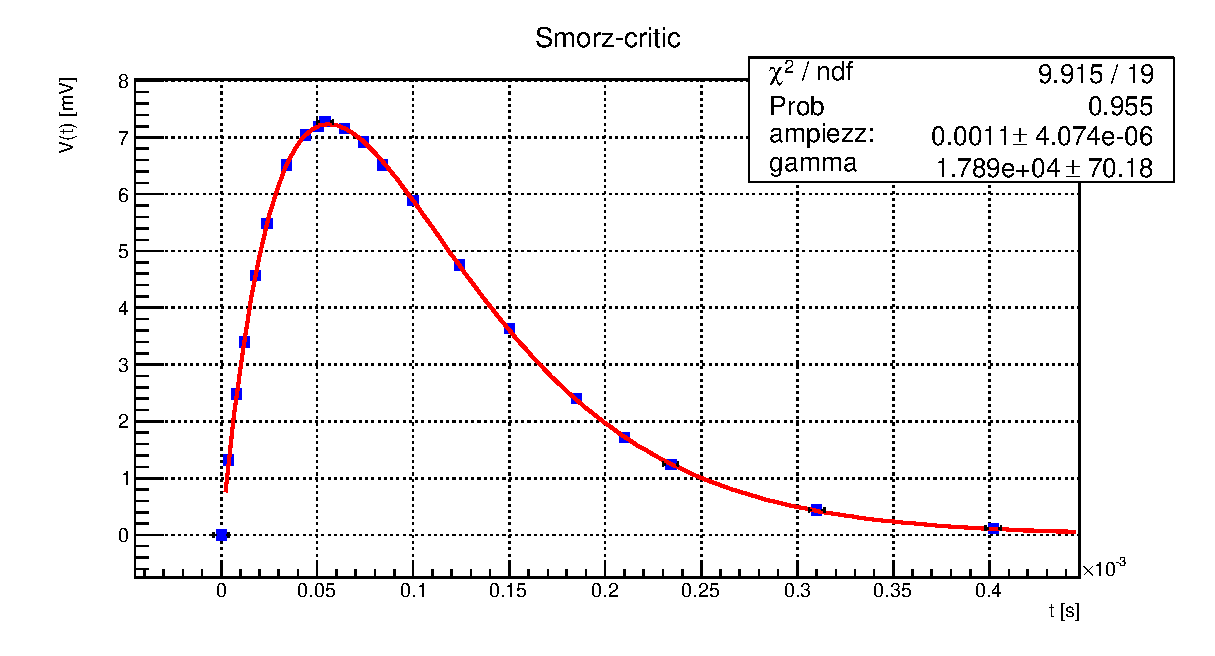
\includegraphics[scale=0.75]{Grafici/C4_P1_Smorz-critic.eps}
\caption{
Circuito RLC serie. Regime di smorzamento critico.
}
\label{fig:C4_P1_critico}
\end{figure}

Nel regime di smorzamento critico non è possibile ottenere una stima puntuale dei parametri $R$, $C$ e $L$ non disponeno di sufficienti equazioni per esprimere i parametri elettrici in funzione di quelli meccanici.

\begin{align*}
    A / V_0 = & RC   \\
    2\gamma    = & R/L   \\
\end{align*}

Le alternative sono: (a) ottenere una misura diretta di $R_{tot}$ misurando la resistenza delle singole componenti con multimetro palmare. Oppure (b) combinare queste misure con altre ottenute negli altri regimi (c) usare la condizione di smorzamento critico

\begin{align*}
    4L = & R^{2}C
\end{align*}

Qui di seguito i risultati ottenuti seguendo il metodo (a):

\begin{table}[H]
\begin{center}
\begin{tabular}{|c|c|c|c|}
\hline

Parametro & Misura & Unità & stima \\ \hline

$R_{tot}$ & diretta & $\Omega$ & $2500\pm1\%$ \\ 

$C$ & indiretta & $nF$ & $87.9\pm2.4\%$ \\ 

$L$ & indiretta & $H$ & $0.069\pm1.4\%$ \\ 

\hline
\end{tabular}
\end{center}
\caption{
Misure indirette dei parametri C e L.
Regime di smorzamento critico.
}
\label{C4_P1_critico_fit}
\end{table}





%%%%%%%%%%%%%%%%%%%%%%%%%%%%%%%%%%%%%%%%%%%%%%%%%%
%%%%%%%%%%%%%%%%%%%%%%%%%%%%%%%%%%%%%%%%%%%%%%%%%%
%%%%%%%%%%% SOVRA



\subsubsection{Regime sovrasmorzato}

Alla condizione che $\omega_0 < \gamma$, il modello teorico per la ddp è

\begin{align*}
V(t) / V_{0} =& A \frac{ \omega_0^2}{2\beta} \; [e^{-(\gamma - \beta)t} - e^{-(\gamma + \beta)t} ] \\
\beta^2 =& \gamma^2 - \omega_0^2 
\end{align*}

Con questa parametrizzazione l'algoritmo di minimizzazione del fit non lineare non converge. Si riparametrizza il modello

\begin{align*}
V(t) / V_{0} =&
Q_{0}  B ( e^{-\theta t} - e^{-\eta t} ) \\
B = & \frac{ (\frac{\eta-\theta}{2})^2 + (\frac{\eta+\theta}{2})^2 }
{\theta + \eta} \\
\theta = & \beta-\gamma \\
\eta   = & \beta+\gamma
\end{align*}

in funzione ora dei tre parametri incogniti $Q_0$, $\eta$ e $\theta$.

\begin{table}[H]
\begin{center}
\begin{tabular}{|c|c|c|c|}
\hline
Tempo & Ddp & Tempo & Ddp \\ \hline
$\mu s$ & $mV$ & $\mu s$ & $mV$ \\ \hline
$\pm 1\%$ & $\pm 80$ & $\pm 1\%$ & $\pm 80$ \\ \hline
0 & 0 & 115 & 8080 \\ \hline
2.6 & 2560 & 180 & 7040 \\ \hline
4.6 & 4640 & 226 & 6320 \\ \hline
9 & 7440 & 340 & 4880 \\ \hline
14.6 & 8960 & 440 & 3920 \\ \hline
28.4 & 9760 & 680 & 2240 \\ \hline
43 & 9520 & 880 & 1440 \\ \hline
65 & 9120 & 1120 & 880 \\ \hline
89 & 8640 & 1870 & 240 \\ \hline
\end{tabular}
\end{center}
\caption{Sovrasmorzato
Resistenza 10.000 (+50+50)   [$\Omega$].
Capacità  46    [$nF$].
Induttore 0.065 [$H$].
}
\label{tab:C4_P1_sovra}
\end{table}

\begin{figure}
\centering
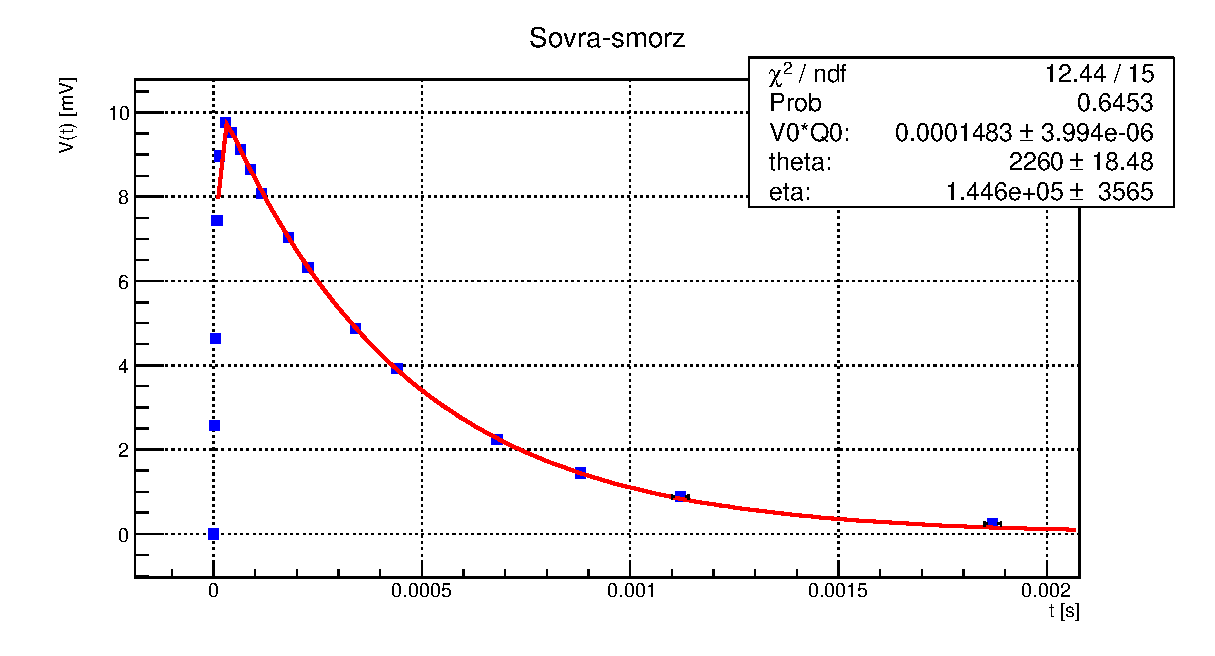
\includegraphics[scale=0.75]{Grafici/C4_P1_Sovra-smorz.eps}
\caption{
Circuito RLC serie. Regime sovrasmorzato.
}
\label{fig:C4_P1_sovra}
\end{figure}

Per ricavare ora i parametri elettrici si possono usare le seguenti relazioni

\begin{align}
&    CR = Q_0  \\
&    \frac{1}{CL} = w_0^2 = \frac{ (\frac{\eta-\theta}{2})^2 + (\frac{\eta+\theta}{2})^2 }
{\theta + \eta} \\
&    \frac{R}{L} = \eta-\theta
\end{align}

Usando una misura diretta di $R$, come fatto anche nei primi due regimi, si ricavano i seguenti risultati per $C$ e $L$ dalla prima e dalla terza relazione.

\begin{table}[H]
\begin{center}
\begin{tabular}{|c|c|c|c|}
\hline

Parametro & Misura & Unità & stima \\ \hline

$R_{tot}$ & diretta & $\Omega$ & $10100\pm1\%$ \\ 

$C$ & indiretta & $nF$ & $2.93\pm4.7\%$ \\ 

$L$ & indiretta & $H$ & $0.07\pm3.5\%$ \\ 

\hline
\end{tabular}
\end{center}
\caption{
Misure indirette dei parametri C e L.
Regime sovrasmorzato.
}
\label{C4_P1_sovra_fit}
\end{table}



\subsubsection{Conclusioni}

Riportiamo per comodità le stime dei parametri $C$ e $L$ risultanti dalle misure condotte nei tre regimi di smorzamento.

\begin{table}[H]
\begin{center}
\begin{tabular}{|c|c|c|c|c|}

\hline
\multicolumn{ 1}{|c}{Parametro} & \multicolumn{ 1}{|c|}{Unità} & \multicolumn{ 3}{c|}{regime} \\ \hline

\multicolumn{ 1}{|c}{} & \multicolumn{ 1}{|c|}{} & sotto & critico & sovra \\ 

$R_{tot}$ & $\Omega$ & $200\pm1\%$ & $2500\pm1\%$ & $10100\pm1\%$ \\ 

$C$ & $nF$ & $46.4\pm3\%$ & $87.9\pm2.4\%$ & $2.93\pm4.7\%$ \\ 

$L$ & $H$ & $0.066\pm2\%$ & $0.069\pm1.4\%$ & $0.07\pm3.5\%$ \\ 

\hline
\end{tabular}
\end{center}
\caption{Confronto risultati di stima nei tre regimi}
\label{C4_P1_finale}
\end{table}


\paragraph{Induttanza} Dai risultati è il parametro più semplice da stimare. Le stime condotte nei tre regimi sono coerenti tra loro, sia nel valore della stima che nel suo errore.

\paragraph{Capacità} La stima della capacità risulta molto più incerta se si opera un confronto tra i risultati ottenuti nei tre regimi. Essendo stati condotti nelle medesime condizioni sperimentali, è possibile che le stime ottenute siano distorte per cause sistematiche legate al modello parametrico utilizzato.

\paragraph{Mispeficiazione del modello}
Una distorsione sistematica delle stime può avvenire perchè alcune ipotesi sottostanti al modello non sono verificate nella pratica.
Nel contesto sperimentale in questione, tale ipotesi di distorsione è sicuramente plausibile per il regime di smorzamento critico, a causa l'impossibilità di intercettare la resistenza critica teorica. All'incertezza sulle stime va perciò aggiunta quella sul regime che effettivamente stanno seguendo i dati.
Per quanto riguarda il regime sotto-smorzato, il rischio di mispecificazione del modello può trovare giustificazione in obiezioni come la non armonicità delle oscillazioni, lo smorzamento non esponenziale. E così anche per il caso sovrasmorzato.

\paragraph{Modello più semplice}
Dei tre regimi, quello sottosmorzato è quello che permette di verificare le ipotesi sottostanti separatamente e con maggior rigore. In ultima analisi è il modello più semplice da testare e anche da stimare. Siccome ognuno dei tre parametri meccanici usati controlla una specifica proprietà dell'andamento dei dati
\begin{itemize}
\item Pulsazione: controlla la periodicità delle oscillazioni.
\item Smorzamento: controlla l'abbattimento dell'ampiezza iniziale.
\item Ampiezza: controlla l'ampiezza iniziale.\\
\end{itemize}

Le tre quantità sarebbero anche potute essere oggetto di stima separatamente una dall'altra, con opportuno rimaneggiamento dei dati. Il vantaggio di stimarle in un unico Fit risiede naturalmente in una miglior stima degli errori e la possibilità di ottenere una misura della bontà di adattamento generale del modello.